\newif\ifglobal

%%%%%%%%%%%%%%%%%%%%%%%
%%% Compile to view %%%
%%%%%%%%%%%%%%%%%%%%%%%

%%%%%%%%%%%%%%%%%%%%%%%%%%%%%%%%%%%%%%%%%%%%%%%%%%%
%%% Readme:                                     %%%
%%% https://www.overleaf.com/read/bwdjvfjksvjy/ %%%
%%%%%%%%%%%%%%%%%%%%%%%%%%%%%%%%%%%%%%%%%%%%%%%%%%%

% >>> M?: marks a module setting number or important notice

% >>> M4: Set {./relative-path} to external files for this module <<<
\def \modulefiles {./43-BITSCRM}
% To add an external file, use:
% (Replace '---' with actual filename)
% '\input{\modulefiles/tables/---.tex}' for tables
% '\includegraphics{\modulefiles/figures/---}' for figures
% '\subfile{\modulefiles/---}' for register files

% >>> M1: This module is in global project? <<<
% 'YES' - uncomment; 'NO' - comment out
\globaltrue

\ifglobal
    \documentclass[main\_\_EN.tex]{subfiles}

\else
    \documentclass[openany, 10pt]{book}

    % >>> M2: In ./00-shared/preamble-trm-module, also find
    %         settings for visibility of todo notes, watermark <<<
    \usepackage{preamble-trm-module}

    % >>> M3: Temporary labels in English,
    %         you can add your own labels there <<<
    \myexternaldocument{./00-shared/temp-labels-en}

\fi %\ifglobal


\setcounter{secnumdepth}{4}


% Define formatting of parts and chapters in text
\titleformat{\chapter}
  [display]
  {\LARGE\bfseries}
  {\color{AllportsColor}Chapter \thechapter}
  {1em}
  {\color{AllportsColor}}
\titlespacing*{\chapter}{0pt}{0pt}{20pt}

% Define headers
\usepackage{fancyhdr}
\usepackage{lipsum}
\renewcommand{\chaptermark}[1]{\markboth{Chapter\, \thechapter\, \ #1}{}}
\fancypagestyle{plain}{%
  \fancyhead{}%
  %\fancyhead[R]{\Navigation}
  \fancyhead[L]{%
    \nouppercase{%
      \ %
      \normalsize\leftmark
    }%
  }%
}
\pagestyle{plain}


% >>> M5: If this module needs any updates in
% './00-shared/preamble-trm-module.sty'
% (include additional package, etc.), contact your module PM
% or create the file './00-shared/changelog.tex' make the
% necessary updates yourself and document them in this file <<<

% Make text left-aligned and allow latex to break pages naturally, comment out for full justification
\raggedright
\raggedbottom


\begin{document}


% Sets language into which pre-defined bits of text are translated
\selectlanguage{english}

% Do not delete this block
\ifglobal
% Add the following front matter if
% this module is outside of global project
\else
    \InputIfFileExists{readme}{}{}
    \listoftodos
    {\let\clearpage\relax \listofdonetodos}
    \tableofcontents
    %\listoftables
    %\listoffigures
\fi


%%%%%%%%%%%%%%%%%%%%%%%%%
%%% TRM Module Begins %%%
%%%%%%%%%%%%%%%%%%%%%%%%%

\hypertarget{bitscrm}{}
\chapter{BitScrambler}
\label{mod:bitscrm}



The \chipname{} has an extensive amount of DMA-capable peripherals (see Chapter \ref{mod:dma} \textit{\nameref{mod:dma}}). These can move data from memory to an external device, and vice versa, without any interference from the CPU. This only works if the external device needs or emits the data in question in the same format as the software expects it: if not, the CPU needs to rewrite the format of the data. Examples include a need to swap bytes, reverse bytes, and shift the data left or right.

As bitwise operations tend to be fairly CPU-expensive and the purpose of DMA is to not use the CPU in the transfer, \chipname{} includes a BitScrambler, which is a dedicated peripheral to change the format of data in between memory and the peripheral. A BitScrambler is capable of performing the aforementioned operations, but as a flexible programmable state machine, it is capable of more advanced things as well. The BitScrambler can be used for memory-to-peripheral,  memory-to-memory, and peripheral-to-memory  transfers.


%%%%%%%%%%%%%%%%%%%%
%%% Introduction %%%
%%%%%%%%%%%%%%%%%%%%

\section{Introduction}

In \chipname{}, a DMA-capable peripheral is one that can read data directly from memory and/or write data directly to memory using a DMA channel. The format this data is read/written in is dependent on the peripheral and generally has only a small amount of flexibility. For most DMA-capable peripherals in \chipname{}, it is possible to attach the BitScrambler to any of these paths for additional flexibility.

When the BitScrambler is attached to a peripheral, it gets the chance to modify any data that flows down a DMA channel associated with that peripheral. Data written to the DMA channel will appear on the BitScrambler input, and what the BitScrambler writes to its output will flow down the DMA channel. The BitScrambler contains instruction memory where instructions on how to route the data between input and output can be stored. As such, by writing an appropriate BitScrambler program, the way the data is rewritten by the BitScrambler can be controlled.

As shown in Figure \ref{fig:bitscrm-blockdia-sys}, the BitScrambler can either be placed in the DMA TX BitScrambler path, where it modifies data flowing from memory to a peripheral, or in the DMA RX BitScrambler path, where it modifies data flowing from a peripheral to memory. It can also be placed in loopback mode, modifying data from memory to memory.




\begin{figure}[H]
\centering
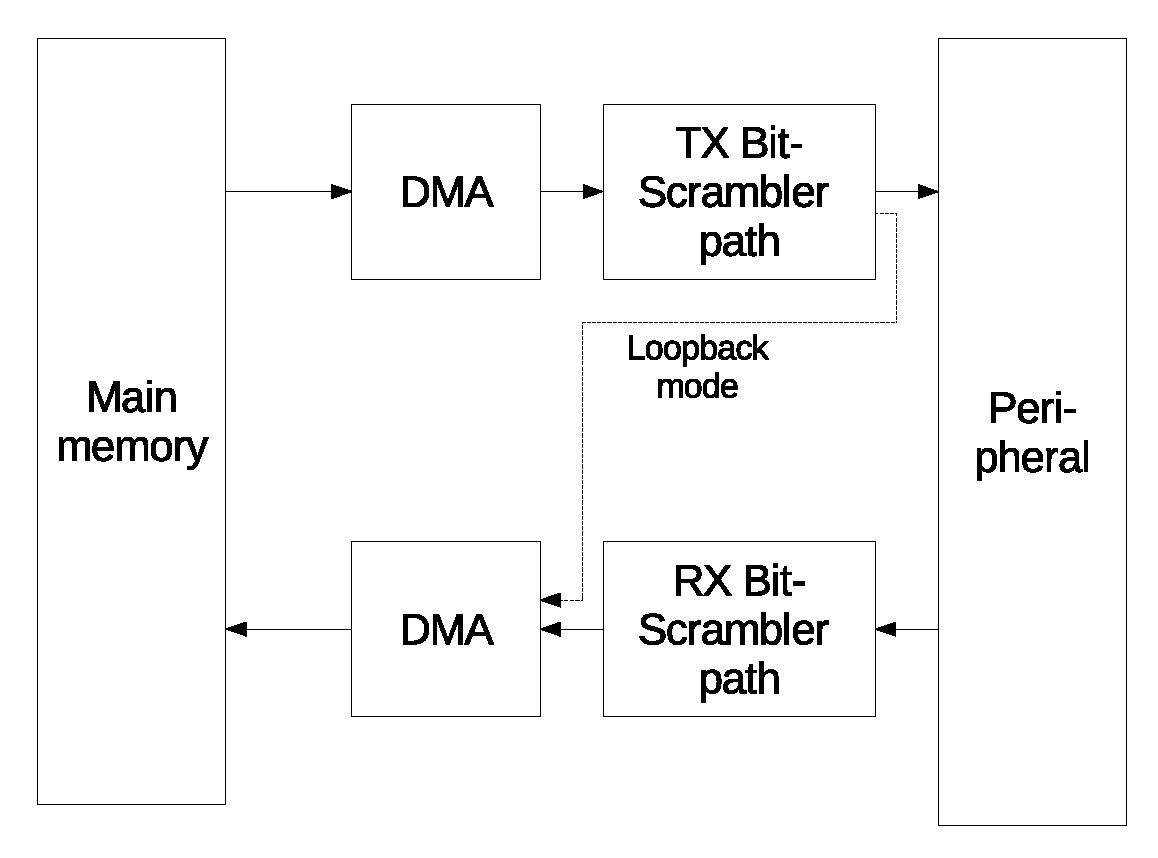
\includegraphics[scale=1.0,width=\textwidth/2]{43-BITSCRM/figures/blockdia_sys}
\caption{BitScrambler System Context Diagram}\label{fig:bitscrm-blockdia-sys}
\end{figure}

%%%%%%%%%%%%%%%%%%%%
%%% Feature List %%%
%%%%%%%%%%%%%%%%%%%%

\section{Feature List}
\label{sec:bitscrm-features}

The BitScrambler has the following features:

\begin{itemize}
    \item One BitScrambler core, which can be used as either a RX (peripheral-to-memory), or TX (memory-to-peripheral) unit
    \item Support for memory-to-memory transfers
    \item Processing up to 32 bits per DMA clock period
    \item Data path controlled by a BitScrambler program stored in instruction memory
    \item Input registers able to read 0, 8, 16, or 32 bits per clock cycle
    \item Output registers:
    \begin{itemize}
        \item Able to write 0, 8, 16, or 32 bits per clock cycle
        \item Data sources for output register bits: 64 bits of input data, two counters, LUT RAM data, data output of last cycle, comparators
        \item With some restrictions, each of the 32 output register bits can come from any bit on the data sources
    \end{itemize}
    \item 8 x 257-bit instruction memory, for storing eight instructions, controlling control flow and the data path
    \item 2048 bytes of lookup table (LUT) memory, configurable as various word widths
\end{itemize}

\section{Application Examples}
\label{sec:bitscrm-app-examples}

\begin{itemize}
    \item Swapping byte, nibble or bit orders in data
    \item Converting palette-based bitmaps to full RGB bitmaps
    \item Run-length encoding or decoding of data
    \item Generating complicated waveforms for e.g. WS2811 chips
\end{itemize}


%%%%%%%%%%%%%%%%%%%%%%%%%%%%%%
%%% Architectural Overview %%%
%%%%%%%%%%%%%%%%%%%%%%%%%%%%%%

\section{Architectural Overview}
\label{sec:bitscrm-arch-overview}


The BitScrambler can be separated into a data path, a control path, and the registers that the CPU can use to program them. The data path moves bits between the incoming DMA stream, internal registers, and the outgoing DMA stream. The control path parses the instructions in the instruction memory to control the data path, as well as handle program flow.


\subsection{Data Path}

\begin{figure}[ht]
\centering
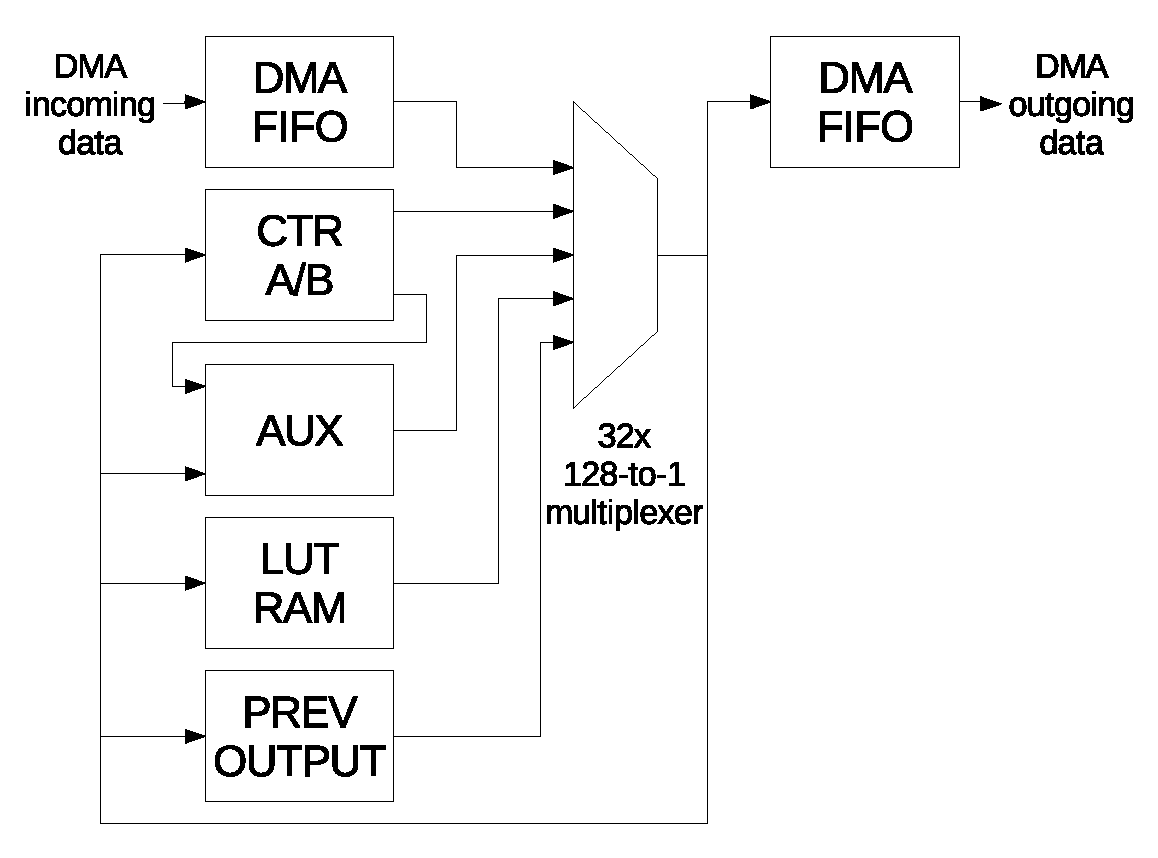
\includegraphics[scale=1.0,width=\textwidth/2]{43-BITSCRM/figures/blockdia_data}
\caption{BitScrambler Data Path Diagram}
\label{fig:bitscrm-blockdia-data}
\end{figure}


The data path of the BitScrambler is intended to take data from the incoming DMA stream, process it according to the program code stored in instruction memory, and write it to the outgoing DMA stream.

\begin{enumerate}
    \item Data is read from the incoming DMA stream into a 64-bit register. At the end of an instruction cycle, as specified in the instruction, N bits (with N being 0, 8, 16, or 32) are read from the DMA stream.
    \item The data in the register is then shifted toward the LSB of the register with the least significant N bits disappearing.
    \item The read data appears as the N most significant bits.
\end{enumerate}

Optionally, on startup, the BitScrambler will automatically read the first 64 bits into this register.

On the other side of the BitScrambler, data is deposited into a 32-bit output register. At the end of the instruction cycle, depending on what the instruction specifies, the least significant 0, 8, 16, or 32 bits will be written to the outgoing DMA stream.

The BitScrambler derives its name from the fact that it can put input bits in any random position in the output, and this is achieved by 32 x 128-to-1 multiplexers. For each of the 32 output register bits, there is one multiplexer that selects the input signals from one of the data sources, dependent on the output of the BitScrambler control path. These data sources are:


\begin{itemize}
\item 64 bits, shifted in from the input FIFO (i.e., the left DMA FIFO block in Figure \ref{fig:bitscrm-blockdia-data}).
As described before, data from the incoming DMA stream is deposited here. In order to facilitate iterating over input bits in a loop, an instruction can enable relative addressing. In this addressing mode, any mux sourcing a bit from the input FIFO register will actually get the bit offset by the counter A register (i.e., CTR A in Figure \ref{fig:bitscrm-blockdia-data}).

\item 32 bits that were sent to the output in the last cycle (i.e., PREV OUTPUT block in Figure \ref{fig:bitscrm-blockdia-data}).
Data sent to the output register will appear on this register one clock cycle later. This allows the BitScrambler to 'remember' data over multiple clock cycles: by outputting a bit to the output register, even if that bit subsequently is not sent to the output FIFO, the next clock cycle can still access it by selecting from this register. Bits can be remembered longer-term by selecting bits from this register for output again, which makes them appear here in the subsequent cycle.


\item 8, 16, or 32 bits that are the output of LUT RAM. The address used to select the data is bit 16 to 24, 25 or 26 of the output data of the last cycle, assuming the LUT width is 32, 16 or 8 bits, respectively.
The LUT RAM is a part of the BitScrambler that takes an address, looks it up in its memory, and outputs the data located at that specific address. The LUT RAM can be filled when the BitScrambler is initialized, but the BitScrambler itself does not have the ability to modify it. Depending on requirements, the LUT RAM can be initialized in the following modes:

\begin{itemize}
    \item 512 x 32-bit words
    \item 1024 x 16-bit words
    \item 2048 x 8-bit words
\end{itemize}

The LUT RAM can be used to do translations of data, e.g. using a calibration curve for a given sensor. It can also be used to implement mathematical functions, with the address input split into two or more input variables and the data output used as the output of the function; the memory should be loaded with the output of the function for each of the input values.

\item 32 bits from 2 x 16-bit counters (i.e., CTR A/B block in Figure \ref{fig:bitscrm-blockdia-data}).
This register contains two 16-bit counters, named 'A' and 'B'. These can be loaded, incremented and decremented via control path instructions.

\item 30 bits from comparators between counter B and the previous data on the output (PREV OUT in Figure \ref{fig:bitscrm-blockdia-data}; the 30 bits described here are part of the AUX block there).
These allow the result of comparisons being used for output or for program flow. This can be useful in e.g. decoding run-length encoded streams, or generating PWM signals.

\item 2 bits, one fixed-high, one fixed-low (i.e., part of AUX in Figure \ref{fig:bitscrm-blockdia-data}).
These are useful if a protocol needs an always-high or always-low bit in the output that does not depend on the input data.
\end{itemize}

Note that some sources cannot be accessed at the same time. Specifically, a given instruction cannot source data from both the high 32 bits of the input FIFO source register as well as the counter registers. When data is read from the LUT, for a LUT that is set to a width of N, the top N bits of both the input FIFO register as well as the top N bits of the counter register become unavailable.


\subsection{Control Path}


\begin{figure}[H]
\centering
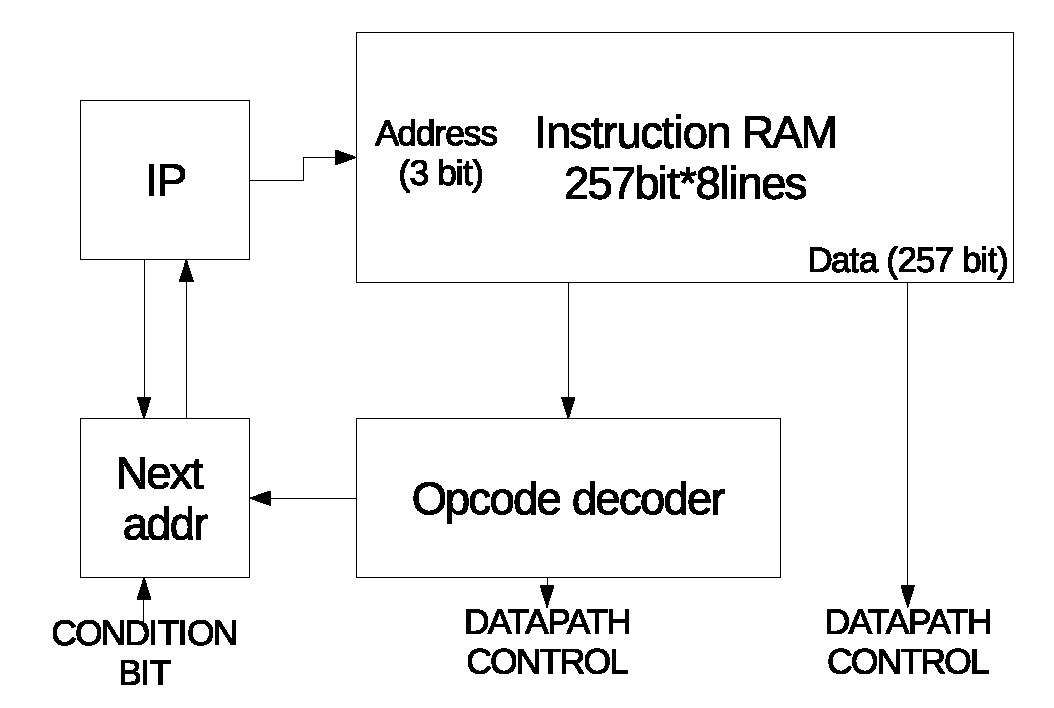
\includegraphics[scale=1.0,width=\textwidth/2]{43-BITSCRM/figures/blockdia_control}
\caption{BitScrambler Control Path Diagram}
\label{fig:bitscrm-blockdia-control}\end{figure}

The BitScrambler behavior is governed by a program stored in instruction RAM. The instruction RAM has space for up to eight instructions, each being 257 bits in size. An instruction configures the data path for the clock cycle the instruction runs in, as well as contains opcodes that control program flow.

A BitScrambler program is similar to a microprocessor program, in that each cycle the BitScrambler will execute the next instruction in instruction memory, unless the opcode tells it to specifically jump to another location. Concretely, this behaviour is implemented using an instruction pointer (IP, see Figure \ref{fig:bitscrm-blockdia-control}), which points to the currently executing instruction. Opcodes can also affect the counter registers.

The bits of the instruction that configure the data path consist of settings for the 32 muxes, as well as some bits to select the availability of the counter bits or LUT output. It also can put the muxes into relative mode, where if they get a bit from the DMA FIFO, the position of that bit is offset by counter B.


%%%%%%%%%%%%%%%%%%%%%%%%%%%%%%
%%% Functional Description %%%
%%%%%%%%%%%%%%%%%%%%%%%%%%%%%%

\section{Functional Description}
\label{sec:bitscrm-func-descr}

The BitScrambler is a flexible device, with its behavior controlled by the program loaded into it as well as the configuration registers that set several global BitScrambler behaviors as well. As such, a BitScrambler program consists of the contents of the 257-bit x 8 instruction RAM as well as the settings for various configuration registers. Both are described below.

\subsection{Instructions}


The 257 bits that make up an instruction are structured as shown in Table \ref{tab:bitscrm-instruction-struct}.

\begin{table}[H]
\centering
\caption{Instruction Structure}
\label{tab:bitscrm-instruction-struct}
\begin{tabular}{ | l | l || l| l | }
\hline\rowcolor{lightgray}
Bit & Field & Bit & Field \\
\hline
0 - 6 & CTL\_MUX\_SEL\_0 & 133 - 139 & CTL\_MUX\_SEL\_19 \\ \hline
7 - 13 & CTL\_MUX\_SEL\_1 & 140 - 146 & CTL\_MUX\_SEL\_20 \\ \hline
14 - 20 & CTL\_MUX\_SEL\_2 & 147 - 153 & CTL\_MUX\_SEL\_21 \\ \hline
21 - 27 & CTL\_MUX\_SEL\_3 & 154 - 160 & CTL\_MUX\_SEL\_22 \\ \hline
28 - 34 & CTL\_MUX\_SEL\_4 & 161 - 167 & CTL\_MUX\_SEL\_23 \\ \hline
35 - 41 & CTL\_MUX\_SEL\_5 & 168 - 174 & CTL\_MUX\_SEL\_24 \\ \hline
42 - 48 & CTL\_MUX\_SEL\_6 & 175 - 181 & CTL\_MUX\_SEL\_25 \\ \hline
49 - 55 & CTL\_MUX\_SEL\_7 & 182 - 188 & CTL\_MUX\_SEL\_26 \\ \hline
56 - 62 & CTL\_MUX\_SEL\_8 & 189 - 195 & CTL\_MUX\_SEL\_27 \\ \hline
63 - 69 & CTL\_MUX\_SEL\_9 & 196 - 202 & CTL\_MUX\_SEL\_28 \\ \hline
70 - 76 & CTL\_MUX\_SEL\_10 & 203 - 209 & CTL\_MUX\_SEL\_29 \\ \hline
77 - 83 & CTL\_MUX\_SEL\_11 & 210 - 216 & CTL\_MUX\_SEL\_30 \\ \hline
84 - 90 & CTL\_MUX\_SEL\_12 & 217 - 223 & CTL\_MUX\_SEL\_31 \\ \hline
91 - 97 & CTL\_MUX\_SEL\_13 & 224 - 249 & OPCODE \\ \hline
98 - 104 & CTL\_MUX\_SEL\_14 & 250 - 251 & CTL\_READ\_IN \\ \hline
105 - 111 & CTL\_MUX\_SEL\_15 & 252 - 253 & CTL\_WR\_OUT \\ \hline
112 - 118 & CTL\_MUX\_SEL\_16 & 254 & CTL\_MUX\_REL \\ \hline
119 - 125 & CTL\_MUX\_SEL\_17 & 255 & CTL\_CTR\_SRC\_SEL \\ \hline
126 - 132 & CTL\_MUX\_SEL\_18 & 256 & CTL\_LUT\_SRC\_SEL \\
\hline
\end{tabular}
\end{table}


The meanings of these fields are as follows:

\begin{itemize}
\item CTL\_MUX\_SEL\_n: This 7-bit field selects the source of bit n in the output register. See Table \ref{tab:bitscrm-ctrmuxsrc} for details.
\item OPCODE: These bits encode an opcode. For the bit pattern of this field, please refer to Table \ref{tab:bitscrm-instruction-opcode}.
\item CTL\_READ\_IN: This selects the number of bits that are read from the input FIFO at the end of the instruction:

\begin{itemize}
\item 0: Do not read any data
\item 1: Read 8 bits
\item 2: Read 16 bits
\item 3: Read 32 bits
\end{itemize}

\item CTL\_WR\_OUT: This selects the number of bits that are written from the output register to the output FIFO at the end of the instruction:
\begin{itemize}
\item 0: Do not write any data
\item 1: Write 8 bits
\item 2: Write 16 bits
\item 3: Write 32 bits
\end{itemize}


\item CTL\_MUX\_REL, CTL\_CTR\_SRC\_SEL and CTR\_LUT\_SRC\_SEL: Select which bits are available to select using the CTL\_MUX\_SEL bits.
\begin{itemize}
    \item CTRL\_CTR\_SRC\_SEL (Control Counter Source Select) makes the bits from counter A and B available
    \item CTL\_LUT\_SRC\_SEL (Control LUT Source Select) makes the output value of the LUT RAM available. See Table \ref{tab:bitscrm-ctrmuxsrc} for details.
    \item When CTL\_MUX\_REL (Control Mux Relative) is 1, the BitScrambler applies the value of counter A as an offset to any CTL\_MUX\_SEL\_n value that is 63 or below. The exact behaviour depends on CTR\_SRC\_SEL, as detailed in Table \ref{tab:bitscrm-ctrmuxrel}.
\end{itemize}

\end{itemize}

\begin{table}[H]
\centering
\caption{Effective CTL\_MUX\_SEL\_n values when CTL\_MUX\_REL is 1}
\label{tab:bitscrm-ctrmuxrel}
\begin{tabular}{|l|l|}
\hline\rowcolor{lightgray}
Condition & Effective value of CTL\_MUX\_SEL \\
\hline
CTL\_MUX\_SEL\_n >= 64 & CTL\_MUX\_SEL (unchanged) \\
CTL\_MUX\_SEL\_n < 64 and CTL\_CTR\_SRC\_SEL = 0 & (CTL\_MUX\_SEL\_n + CTRA) \& 63 \\
CTL\_MUX\_SEL\_n < 31 and CTL\_CTR\_SRC\_SEL = 1 & (CTL\_MUX\_SEL\_n + CTRA) \& 31 \\
32 <= CTL\_MUX\_SEL\_n < 64 and CTL\_CTR\_SRC\_SEL = 1 & ((CTL\_MUX\_SEL\_n + CTRA) \& 31) + 32 \\
\hline
\end{tabular}
\end{table}


Of these fields, most are data path configuration items. The field that affects the control path is OPCODE, although CTL\_MUX\_REL, CTL\_CTR\_SRC\_SEL, and CTR\_LUT\_SRC\_SEL may influence how some of the opcodes work by adjusting the source selection for the IF/IFN opcodes.

CTL\_MUX\_SEL\_n: These fields, one for each bit in the output register, select the source for that particular bit. The specific bit chosen is partially dependent on the settings of the CTL\_MUX\_REL, CTL\_CTR\_SRC\_SEL, and CTR\_LUT\_SRC\_SEL. Given CTL\_MUX\_SRC\_n has value N, the bit is selected as described in Table \ref{tab:bitscrm-ctrmuxsrc}. Note that the source selection for IF/IFN opcodes is affected in the same way.


\begin{longtable}{ | p{3cm} | p{13cm} | }
\caption{CTL\_MUX\_SEL Values} \label{tab:bitscrm-ctrmuxsrc} \\
\hline\rowcolor{lightgray}
Bit & Description \\ \hline
\endfirsthead
\hline\rowcolor{lightgray}
Bit & Description \\
\hline
\endhead
0-31 & The bit is sourced from bit N in the incoming FIFO register. \\
\hline
\multirow{4}{4em}{32-63} & The source of the bit depends on the setting of CTL\_CTR\_SRC\_SEL and
CTR\_LUT\_SRC\_SEL: \\
& If CTL\_CTR\_SRC\_SEL = 0: the bit is sourced from bit N in the incoming FIFO register.\\
& If CTL\_CTR\_SRC\_SEL = 1: the bit is sourced from bit (N-32) of the counter registers. Specifically, if N is 32 to 47, the bit is sourced from bit (N-32) of counter A and if N is 48 to 63, the bit is sourced from bit (N-48) of counter B. \\
& If CTL\_LUT\_SRC\_SEL = 1: Depending on the width of the LUT (8, 16, or 32 bits), a read of the top 8, 16, or 32 bits will return data from the LUT rather than what CTL\_CTR\_SRC\_SEL selects. Specifically, given a LUT width of N, 63 will return LUT output bit (N-1), 62 will return LUT output bit (N-2) and so on.\\
\hline
64 & CounterB[7:0] =< last[7:0] \\
65 & CounterB[7:0] > last[7:0] \\
66 & CounterB[7:0] = last[7:0] \\
67 & CounterB[7:0] =< last[15:8] \\
68 & CounterB[7:0] > last[15:8] \\
69 & CounterB[7:0] = last[15:8] \\
70 & CounterB[7:0] =< last[23:16] \\
71 & CounterB[7:0] > last[23:16] \\
72 & CounterB[7:0] = last[23:16] \\
73 & CounterB[7:0] =< last[31:24] \\
74 & CounterB[7:0] > last[31:24] \\
75 & CounterB[7:0] = last[31:24] \\
76 & CounterB[15:8] =< last[7:0] \\
77 & CounterB[15:8] > last[7:0] \\
78 & CounterB[15:8] = last[7:0] \\
79 & CounterB[15:8] =< last[15:8] \\
80 & CounterB[15:8] > last[15:8] \\
81 & CounterB[15:8] = last[15:8] \\
82 & CounterB[15:8] =< last[23:16] \\
83 & CounterB[15:8] > last[23:16] \\
84 & CounterB[15:8] = last[23:16] \\
85 & CounterB[15:8] =< last[31:24] \\
86 & CounterB[15:8] > last[31:24] \\
87 & CounterB[15:8] = last[31:24] \\
88 & CounterB[15:0] =< last[15:0] \\
89 & CounterB[15:0] > last[15:0] \\
90 & CounterB[15:0] = last[15:0] \\
91 & CounterB[15:0] =< last[31:16] \\
92 & CounterB[15:0] > last[31:16] \\
93 & CounterB[15:0] = last[31:16] \\
94 & Always 0 \\
95 & Always 1 \\
\hline
96-127 & The bits selected here are the same as the bits on the output register at the end of the previous cycle. \\
\hline
\end{longtable}

The BitScrambler recognizes seven opcodes, which are encoded in the opcode fields as shown in Table \ref{tab:bitscrm-instruction-opcode}.

\bgroup
\setlength{\tabcolsep}{0.4em}
\begin{table}[H]
\centering
\caption{Instruction Opcode}
\label{tab:bitscrm-instruction-opcode}
\begin{tabular}{|l|c|c|c|c|c|c|c|c|c|c|c|c|c|c|c|c|c|c|c|c|c|c|c|c|c|c|}
\hline\rowcolor{lightgray}
\backslashbox{Opcode}{Bit} & 25 & 24 & 23 & 22 & 21 & 20 & 19 & 18 & 17 & 16 & 15 & 14 & 13 & 12 & 11 & 10 & 9 & 8 & 7 & 6 & 5 & 4 & 3 & 2 & 1 & 0 \\
\hline
LOOP & 1 & c & \multicolumn{3}{|c|}{tgt} & \multicolumn{16}{|c|}{end\_val} & \multicolumn{5}{|c|}{ctr\_add}  \\
\hline
ADD & 0 & c & h & l & 0 & 0 & 0 & 0 & 0 & 0 & \multicolumn{16}{|c|}{ctr\_add} \\
\hline
IF & 0 & 0 & \multicolumn{3}{|c|}{tgt} & 0 & 0 & 0 & 0 & 1 & 0 & 0 & 0 & 0 & 0 & 0 & 0 & 0 & 0 & \multicolumn{7}{|c|}{src} \\
\hline
IFN & 0 & 0 & \multicolumn{3}{|c|}{tgt} & 0 & 0 & 0 & 1 & 0 & 0 & 0 & 0 & 0 & 0 & 0 & 0 & 0 & 0 & \multicolumn{7}{|c|}{src} \\
\hline
LDCTD & 0 & c & h & l & 0 & 0 & 0 & 0 & 1 & 1 & \multicolumn{16}{|c|}{ctr\_set} \\
\hline
LDCTI & 0 & c & h & l & 0 & 0 & 0 & 1 & 0 & 0 & 0 & 0 & 0 & 0 & 0 & 0 & 0 & 0 & 0 & 0 & 0 & 0 & 0 & 0 & 0 & 0 \\
\hline
ADDCTI & 0 & c & h & l & 0 & 0 & 0 & 1 & 0 & 1 & 0 & 0 & 0 & 0 & 0 & 0 & 0 & 0 & 0 & 0 & 0 & 0 & 0 & 0 & 0 & 0 \\
\hline
\end{tabular}
\end{table}
\egroup

The fields are defined as follows:


\begin{itemize}\item c: Configures which counter to use.
\begin{itemize}
    \item 0: counter A
    \item 1: counter B
\end{itemize}
\item end\_val, ctr\_add, ctr\_set: 16-bit (or 5-bit) value. Please refer to the instruction descriptions below for the meanings of these fields.
\item tgt: The location of an instruction. Range: 0 \verb+~+ 7.
\item h: 1 if the upper 8 bits need to be written back to a counter (if the opcode ends with -H).
\item l: 1 if the lower 8 bits need to be written back to a counter (if the opcode ends with -L).
\end{itemize}


Note that if an opcode does not specify H or L, it is assumed that the full 16 bits need to be written back and the h and l bits will both be 1.

These seven opcodes affect the state of the BitScrambler as follows:

\begin{table}[H]
\caption{LOOP Opcode}
\label{tab:bitscrm-loop-opcode}
\begin{tabular}{|l|l|}
\hline
\multicolumn{2}{|l|}{\texttt{LOOPc end\_val, ctr\_add, tgt}} \\
\hline
\multicolumn{2}{|L{17cm}|}{Loop on counter indicated by c, add ctr\_add to the counter, and loop back to tgt until the counter reaches end\_val. When that happens, reset the counter and fall through.} \\
\hline
\multirow{4}{*}{Argument} & c: Either A or B, indicates counter to use \\
& tgt: 3-bit target instruction addresses \\
& end\_val: 16-bit value to compare the counter to \\
& ctr\_add: 5-bit signed value to add to the counter \\
\hline
\multirow{7}{*}{Pseudo-code} & \texttt{if ((unsigned)ctrC < end\_val) begin} \\
& \hspace*{4mm} \texttt{IP <= tgt} \\
& \hspace*{4mm} \texttt{ctr\_c <= ctr\_c + sign\_extend(ctr\_add)} \\
& \texttt{end else begin} \\
& \hspace*{4mm} \texttt{IP <= IP + 1} \\
& \hspace*{4mm} \texttt{ctr\_c <= 0} \\
& \texttt{end} \\
\hline
\end{tabular}
\end{table}

\begin{table}[H]
\caption{ADD Opcode}
\label{tab:bitscrm-add-opcode}
\begin{tabular}{|l|l|}
\hline
\multicolumn{2}{|l|}{\texttt{ADDc[H|L] ctr\_add}} \\
\hline
\multicolumn{2}{|L{17cm}|}{Add immediate value to counter indicated by c, and optionally write back only upper or lower 8 bits.} \\
\hline
\multirow{4}{*}{Argument} & c: Either A or B, indicate counter to use \\
& ctr\_add: 16-bit value to add to counter \\
& If opcode is ADDcH, only most significant 8 bits are written back \\
& If opcode is ADDcL, only least-significant 8 bits are written back \\
& If opcode is ADDc, all 16 bits will be written back (h=1, l=1). \\
\hline
\multirow{7}{*}{Pseudo-code} & \texttt{tmp <= ctr\_c + ctr\_add} \\
& \texttt{if (h) begin} \\
& \hspace*{4mm} \texttt{ctr\_c[15:8] <= tmp[15:8]} \\
& \texttt{end} \\
& \texttt{if (l) begin} \\
& \hspace*{4mm} \texttt{ctr\_c[7:0] <= tmp[7:0]} \\
& \texttt{end} \\
& \texttt{IP <= IP + 1} \\
\hline
Note & The NOP (no operation) pseudo-op is encoded as ‘ADDA 0’. \\
\hline
\end{tabular}
\end{table}

\begin{table}[H]
\caption{IF Opcode}
\label{tab:bitscrm-if-opcode}
\begin{tabular}{|l|p{14cm}|}
\hline
\multicolumn{2}{|l|}{\texttt{IF ctl\_cond\_src, tgt}} \\
\hline
\multicolumn{2}{|L{17cm}|}{Jump to target if the indicated mux source bit is set.} \\
\hline
\multirow{2}{*}{Argument} & ctl\_cond\_src: Mux source (see \hyperref[tab:bitscrm-ctrmuxsrc]{CTR\_MUX\_SRC sources}) \\
& tgt: 3-bit target instruction addresses  \\
\hline
\multirow{5}{*}{Pseudo-code} & \texttt{if (ctl\_cond\_src) begin} \\
& \hspace*{4mm} \texttt{IP <= tgt} \\
& \texttt{end else begin} \\
& \hspace*{4mm} \texttt{IP <= IP + 1} \\
& \texttt{end} \\
\hline
Note & The JMP (always jump) pseudo-op is implemented as an ‘IF 95,tgt’ opcode, using the always-1 bit from the AUX bits. \\
\hline
\end{tabular}
\end{table}

\begin{table}[H]
\caption{IFN Opcode}
\label{tab:bitscrm-ifn-opcode}
\begin{tabular}{|l|l|}
\hline
\multicolumn{2}{|l|}{\texttt{IFN ctl\_cond\_src, tgt}} \\
\hline
\multicolumn{2}{|L{17cm}|}{Jump to target if the indicated mux source bit is NOT set (note: same as IF but condition is negated).} \\
\hline
\multirow{2}{*}{Argument} & ctl\_cond\_src: Mux source (see \hyperref[tab:bitscrm-ctrmuxsrc]{CTR\_MUX\_SRC sources}) \\
& tgt: 3-bit target instruction addresses \\
\hline
\multirow{5}{*}{Pseudo-code} & \texttt{if (ctl\_cond\_src) begin} \\
& \hspace*{4mm} \texttt{IP <= IP + 1} \\
& \texttt{end else begin} \\
& \hspace*{4mm} \texttt{IP <= tgt} \\
& \texttt{end} \\
\hline
\end{tabular}
\end{table}


\begin{table}[H]
\caption{LDCTD Opcode}
\label{tab:bitscrm-ldctd-opcode}
\begin{tabular}{|l|l|}
\hline
\multicolumn{2}{|l|}{\texttt{LDCTDc[H|L] ctr\_set}} \\
\hline
\multicolumn{2}{|L{17cm}|}{Load counter direct (from immediate), and optionally only load high or low 8 bits of counter.} \\
\hline
\multirow{4}{*}{Argument} & c: Either A or B, indicate counter to use \\
& ctr\_set: 16-bit value to set the counter to \\
& h: if opcode is LDCTDcH, only most significant 8 bits are set \\
& l: if opcode is LDCTDcL, only least-significant 8 bits are set \\
& If opcode is LDCTDc, all 16 bits are set (h=1, l=1)\\
\hline
\multirow{7}{*}{Pseudo-code} & \texttt{if (h) begin} \\
& \hspace*{4mm} \texttt{ctr\_c[15:8] <= ctr\_set[15:8]} \\
& \texttt{end} \\
& \texttt{if (l) begin} \\
& \hspace*{4mm} \texttt{ctr\_c[7:0] <= ctr\_set[7:0]} \\
& \texttt{end} \\
& \texttt{IP <= IP + 1} \\
\hline
\end{tabular}
\end{table}

\begin{table}[H]
\caption{LDCTI Opcode}
\label{tab:bitscrm-ldcti-opcode}
\begin{tabular}{|l|l|}
\hline
\multicolumn{2}{|l|}{\texttt{LDCTIc[H|L]}} \\
\hline
\multicolumn{2}{|L{17cm}|}{Load counter indirect (from most significant 16 bits of mux output), and optionally only load high or low 8 bits of counter.} \\
\hline
\multirow{3}{*}{Argument} & c: Either A or B, indicate counter to use \\
& h: If opcode is LDCTIcH, only the most significant 8 bits are set\\
& l: If opcode is LDCTIcL, only the least significant 8 bits are set \\
& If opcode is LDCTIc, all 16 bits are set (h=1, l=1) \\
\hline
\multirow{7}{*}{Pseudo-code} & \texttt{if (h) begin} \\
& \hspace*{4mm} \texttt{ctr\_c[15:8] <= mux\_out[31:24]} \\
& \texttt{end} \\
& \texttt{if (l) begin} \\
& \hspace*{4mm} \texttt{ctr\_c[7:0] <= mux\_out[23:16]} \\
& \texttt{end} \\
& \texttt{IP <= IP + 1} \\
\hline
\end{tabular}
\end{table}

\begin{table}[H]
\caption{ADDCTI Opcode}
\label{tab:bitscrm-addcti-opcode}
\begin{tabular}{|l|l|}
\hline
\multicolumn{2}{|l|}{\texttt{ADDCTIc[H|L]}} \\
\hline
\multicolumn{2}{|L{17cm}|}{Add indirect (from most significant 16 bits of mux output) value to counter. Optionally only add to high or low 8 bits of counter.} \\
\hline
\multirow{7}{*}{Argument} & c: Either A or B, indicate counter to use \\
& h: If opcode is ADDCTIcH, bit 24 to 31 of the output mux are added to the most significant 8 \\
& bits of the counter \\
& l: If opcode is ADDCTIcL, bit 16 to 23 of the output mux are added to the least significant 8 \\
& bits of the counter \\
& If opcode is ADDCTIc, bit 16 to 31 of the output mux are added to all 16 bits of the counter \\
& (h=1, l=1) \\
\hline
\multirow{7}{*}{Pseudo-code} & \texttt{if (h) begin} \\
& \hspace*{4mm} \texttt{ctr\_c[15:8] <= ctr\_c[15:8] + mux\_out[31:24]} \\
& \texttt{end else if (l) begin} \\
& \hspace*{4mm} \texttt{ctr\_c[7:0] <= ctr\_c[7:0] + mux\_out[23:16]} \\
& \texttt{end else begin} \\
& \hspace*{4mm} \texttt{ctr\_c[15:0] <= ctr\_c[15:0] + mux\_out[31:16]} \\
& \texttt{end} \\
& \texttt{IP <= IP + 1} \\
\hline
\end{tabular}
\end{table}

\subsection{Configuration Registers}

The BitScrambler is configured using a set of registers. Specifically, these registers are used to write a program into BitScrambler, write its LUT RAM, configure its behaviour, and start and stop BitScrambler operation. They are also used to attach a BitScrambler to a peripheral DMA path.

The \chipname{} only has one BitScrambler core which can either be placed in the TX path (where data is sent from the memory to a peripheral) or in a RX path (where data is sent from the peripheral to memory). For compatibility with other ESP series chips, when the BitScrambler core is placed in the TX path, it is controlled with the registers prefixed by BITSCRAMBLER\_TX\_ while when it is placed in the RX path, the registers prefixed by BITSCRAMBLER\_RX\_ govern its behaviour. Which path is active is decided by \hyperref[fielddesc:BITSCRAMBLERRXENA]{BITSCRAMBLER\_RX\_ENA} and
\hyperref[fielddesc:BITSCRAMBLERTXENA]{BITSCRAMBLER\_TX\_ENA}, of which only one is allowed to be active at any given time.

\begin{tiplisting}
For convenience, in this section we will refer to the TX path registers only; to get the RX path register descriptions, simply swap the prefixes.
\end{tiplisting}


When modifying the input or output of a peripheral, the BitScrambler needs to be attached to the DMA path of that peripheral. To do this, write the appropriate value for the peripheral into the HP\_SYSTEM\_BITSCRAMBLER\_PERI\_TX\_SEL or HP\_SYSTEM\_BITSCRAMBLER\_PERI\_RX\_SEL field of the HP\_SYSTEM\_BITSCRAMBLER\_PERI\_SEL\_REG register.

The  BitScrambler can also run in memory-to-memory mode. For this, the \hyperref[fielddesc:BITSCRAMBLERLOOPMODE]{BITSCRAMBLER\_LOOP\_MODE} bit in \hyperref[regdesc:BITSCRAMBLERSYSREG]{BITSCRAMBLER\_SYS\_REG} needs to be set to one. In this mode, the TX BitScrambler is put into loopback mode while the RX BitScrambler is unused and unavailable. The BitScrambler still needs to be attached to a peripheral (although the peripheral does not need to be configured); the DMA path for this peripheral will be unusable.

Neither the program memory nor the LUT RAM are accessible to the main processor directly. Rather, they need to be written indirectly, by setting an address in one register and then writing the data in a second register.

Specifically, for the LUT RAM, the address is written in the \hyperref[fielddesc:BITSCRAMBLERTXLUTIDX]{BITSCRAMBLER\_TX\_LUT\_IDX} field of \hyperref[regdesc:BITSCRAMBLERTXLUTCFG0REG]{BITSCRAMBLER\_TX\_LUT\_CFG0\_REG} and the data is written to or read from \hyperref[regdesc:BITSCRAMBLERTXLUTCFG1REG]{BITSCRAMBLER\_TX\_LUT\_CFG1\_REG}. The width of the LUT, as visible to the BitScrambler, can be configured using the \hyperref[fielddesc:BITSCRAMBLERTXLUTMODE]{BITSCRAMBLER\_TX\_LUT\_MODE} field. Note that when the host processor writes to the LUT in the aforementioned fashion, the addressing and data size needs to adhere to the configured LUT width.

Similarly, the instruction memory is written by setting the address up in \hyperref[regdesc:BITSCRAMBLERTXINSTCFG0REG]{BITSCRAMBLER\_TX\_INST\_CFG0\_REG} and writing the data to or reading it from \hyperref[regdesc:BITSCRAMBLERTXINSTCFG1REG]{BITSCRAMBLER\_TX\_INST\_CFG1\_REG}. As the BitScrambler instructions are 257 bits, one instruction needs to be written as 9 32-bit words (with the 257th bit being in the LSB of the 9th word). To achieve that purpose, the \hyperref[regdesc:BITSCRAMBLERTXINSTCFG0REG]{BITSCRAMBLER\_TX\_INST\_CFG0\_REG} register is divided into two fields. The position of the instruction is written into the \hyperref[fielddesc:BITSCRAMBLERTXINSTIDX]{BITSCRAMBLER\_TX\_INST\_IDX} field while the word offset within the instruction is written to \hyperref[fielddesc:BITSCRAMBLERTXINSTPOS]{BITSCRAMBLER\_TX\_INST\_POS}.

As the BitScrambler has the ability to generate more or less data than it gets on the input, a BitScrambler-controlled DMA stream can end in one or two ways. The first is that the receiver (either memory in case of the RX BitScrambler, or the peripheral in case of the TX BitScrambler) stops accepting data because it is configured to only receive a limited number of bytes. This case is pretty simple: the BitScrambler will simply halt as it cannot write any more data. The other way is that the transmitter (the peripheral for the RX BitScrambler and the memory for the TX BitScrambler) stops sending data. This is a more complicated situation, as the BitScrambler may or may not be processing some data that needs to be written to the output.

In order to allow the BitScrambler to send out the data it is still processing, two methods have been devised to handle a certain amount of data after the input data stream has ended. Both depend on setting \hyperref[regdesc:BITSCRAMBLERRXTAILINGBITSREG]{BITSCRAMBLER\_RX\_TAILING\_BITS\_REG} to a certain value N:

\begin{itemize}
\item EOF-on-N-reads: After the input data stream ends, the BitScrambler reads N dummy bytes from the input. The value of these bytes is zero. After the Nth byte is read, the BitScrambler halts and the DMA stream ends.

\item EOF-on-N-writes: After the input data stream ends, the BitScrambler is allowed to write N more bytes to the output. During this time, any reads on the input stream return zero-value dummy bytes. After the N'th byte is written, the BitScrambler halts and the DMA stream ends.
\end{itemize}

To configure either mode, set the option bits as follows:

\begin{table}[H]
\centering
\caption{Settings for EOF modes}
\label{tab:bitscrm-settings-for-eof-modes}
\begin{tabular}{|l|c|c|}
\hline\rowcolor{lightgray}
Register & EOF-on-N-reads & EOF-on-N-writes \\
\hline
\hyperref[fielddesc:BITSCRAMBLERTXRDDUMMY]{BITSCRAMBLER\_TX\_RD\_DUMMY} & 1 & 1 \\ \hline
\hyperref[fielddesc:BITSCRAMBLERTXFETCHMODE]{BITSCRAMBLER\_TX\_FETCH\_MODE} & 0 & 0 \\ \hline
\hyperref[fielddesc:BITSCRAMBLERTXEOFMODE]{BITSCRAMBLER\_TX\_EOF\_MODE} & 1 & 0 \\ \hline
\hyperref[fielddesc:BITSCRAMBLERTXHALTMODE]{BITSCRAMBLER\_TX\_HALT\_MODE} & 1 & 1 \\\hline
\end{tabular}
\end{table}

%%%%%%%%%%%%%%%%%%%%%%%%%%%%%%
%%% Programming Procedures %%%
%%%%%%%%%%%%%%%%%%%%%%%%%%%%%%

\section{Programming Procedures}
\label{sec:bitscrm-prog-procedures}

Note that these instructions are written for a BitScrambler with the TX path enabled, either in the memory-to-peripheral path, or memory-to-memory path if in loopback mode. For the peripheral-to-memory path, the RX path is used. Unless otherwise indicated, you can exchange "TX" for "RX" in these instructions to configure the RX path.


\begin{enumerate}
    \item Attach the BitScrambler to a peripheral by configuring HP\_SYSTEM\_BITSCRAMBLER\_PERI\_TX\_SEL field in HP\_SYSTEM\_BITSCRAMBLER\_PERI\_SEL\_REG register. Note that this step is required even in loopback mode.
    \item Enable the BitScrambler by setting the \hyperref[fielddesc:BITSCRAMBLERTXENA]{BITSCRAMBLER\_TX\_ENA} field in the \hyperref[regdesc:BITSCRAMBLERTXCTRLREG]{BITSCRAMBLER\_TX\_CTRL\_REG} register. Make sure only one of \hyperref[fielddesc:BITSCRAMBLERTXENA]{BITSCRAMBLER\_TX\_ENA} and \hyperref[fielddesc:BITSCRAMBLERRXENA]{BITSCRAMBLER\_RX\_ENA} is set at any time.
    \item Configure loopback mode if required. If loopback mode is needed, set \hyperref[fielddesc:BITSCRAMBLERLOOPMODE]{BITSCRAMBLER\_LOOP\_MODE} in the \hyperref[regdesc:BITSCRAMBLERSYSREG]{BITSCRAMBLER\_SYS\_REG} register. Otherwise, clear it.
    \item Load program into BitScrambler. For each instruction and each 32-bit word within the instruction, set the \hyperref[fielddesc:BITSCRAMBLERTXINSTIDX]{BITSCRAMBLER\_TX\_INST\_IDX} and \hyperref[fielddesc:BITSCRAMBLERTXINSTPOS]{BITSCRAMBLER\_TX\_INST\_POS} fields in the \hyperref[regdesc:BITSCRAMBLERTXINSTCFG0REG]{BITSCRAMBLER\_TX\_INST\_CFG0\_REG} register, then write the word in the \hyperref[regdesc:BITSCRAMBLERTXINSTCFG1REG]{BITSCRAMBLER\_TX\_INST\_CFG1\_REG} register. Note that the 257th bit is written as bit 0 into \hyperref[regdesc:BITSCRAMBLERTXINSTCFG1REG]{BITSCRAMBLER\_TX\_INST\_CFG1\_REG}.
    \item Load LUT into BitScrambler, if needed:
    \begin{enumerate}
        \item Configure \hyperref[fielddesc:BITSCRAMBLERTXLUTMODE]{BITSCRAMBLER\_TX\_LUT\_MODE} in \hyperref[regdesc:BITSCRAMBLERTXLUTCFG0REG]{BITSCRAMBLER\_TX\_LUT\_CFG0\_REG} to set the LUT width
        \item Write the address to the \hyperref[regdesc:BITSCRAMBLERTXLUTCFG0REG]{BITSCRAMBLER\_TX\_LUT\_CFG0\_REG}
        \item Write the data word or the byte itself to \hyperref[regdesc:BITSCRAMBLERTXLUTCFG1REG]{BITSCRAMBLER\_TX\_LUT\_CFG1\_REG}
    \end{enumerate}
        Note that it is acceptable to change the LUT width after writing the data and before starting the BitScrambler.
    \item Configure BitScrambler. Dependent on what the BitScrambler program expects, you may need to set or clear the various bits in the \hyperref[regdesc:BITSCRAMBLERTXCTRLREG]{BITSCRAMBLER\_TX\_CTRL\_REG} register. You may also need to set \hyperref[regdesc:BITSCRAMBLERTXTAILINGBITSREG]{BITSCRAMBLER\_TX\_TAILING\_BITS\_REG} to an applicable value.
    \item Start the BitScrambler by clearing the \hyperref[fielddesc:BITSCRAMBLERTXHALT]{BITSCRAMBLER\_TX\_HALT} bit in the \hyperref[regdesc:BITSCRAMBLERTXCTRLREG]{BITSCRAMBLER\_TX\_CTRL\_REG} register.
    \item Start DMA transaction. Please refer to Chapter \ref{mod:dma} \textit{\nameref{mod:dma}} for more information about DMA subsystem and refer to the peripheral chapter if loopback mode is not used.
    \item Wait until DMA transaction is done.
    \item Halt the BitScrambler by setting the \hyperref[fielddesc:BITSCRAMBLERTXHALT]{BITSCRAMBLER\_TX\_HALT} in the \hyperref[regdesc:BITSCRAMBLERTXCTRLREG]{BITSCRAMBLER\_TX\_CTRL\_REG} register.
    \item Wait for halt state. The BitScrambler is halted when the \hyperref[fielddesc:BITSCRAMBLERTXINIDLE]{BITSCRAMBLER\_TX\_IN\_IDLE} bit in the \hyperref[regdesc:BITSCRAMBLERTXSTATEREG]{BITSCRAMBLER\_TX\_STATE\_REG} register is set.
    \item Reset the FIFO by writing 1 and then 0 to the \hyperref[fielddesc:BITSCRAMBLERTXFIFORST]{BITSCRAMBLER\_TX\_FIFO\_RST} bit in the \hyperref[regdesc:BITSCRAMBLERTXCTRLREG]{BITSCRAMBLER\_TX\_CTRL\_REG} register.
    \item The BitScrambler is ready for a new transaction with the current program and LUT configuration. Simply start from step 7 to do this.
\end{enumerate}



% >>> If your module has no registers, delete sample text
%       for Sections Register Summary and Registers below <<<

%%%%%%%%%%%%%%%%%%%%%%%%
%%% Register Summary %%%
%%%%%%%%%%%%%%%%%%%%%%%%

% >>> Update the sample text below and insert
%     the info on register summary into the subfile <<<

\newpage
\hypertarget{bitscrm-reg-summ}{}
\section{Register Summary}
\label{sec:bitscrm-reg-summ}

The addresses in this section are relative to the Bit-scrambler base address provided in Table \ref{tab:sysmem-base-address} in Chapter \ref{mod:sysmem} \textit{\nameref{mod:sysmem}}.

The abbreviations given in Column \textbf{Access} are explained in Section \hyperref[glossary-access-types]{\textit{Access Types for Registers}}.

\subfile{\modulefiles/43-BITSCRM-reg-summ__EN}


%%%%%%%%%%%%%%%%%
%%% Registers %%%
%%%%%%%%%%%%%%%%%

% >>> Update the sample text below and insert
%      the info on registers into the subfile <<<

\newpage
\section{Registers}

The addresses in this section are relative to the Bit-scrambler base address provided in Table \ref{tab:sysmem-base-address} in Chapter \ref{mod:sysmem} \textit{\nameref{mod:sysmem}}.

For how to program reserved fields, please refer to Section \hyperref[programming-reserved-field]{Programming Reserved Register Field}.

\subfile{\modulefiles/43-BITSCRM-reg__EN}


\end{document}
